\documentclass[12pt]{article}
\usepackage{tabularx}
\usepackage{amsmath} 
\usepackage{graphicx}
\usepackage[margin=1in]{geometry}
\usepackage{cite}
\usepackage[final]{hyperref}
\hypersetup{
	colorlinks=true,      
	linkcolor=blue,       
	citecolor=blue,       
	filecolor=magenta,    
	urlcolor=blue         
}
\usepackage{blindtext}
\usepackage{amssymb}
\usepackage{esint}
\usepackage{tikz}
\usepackage{pgfplots}
\usepackage{gensymb}
\usetikzlibrary{datavisualization}
\usetikzlibrary{datavisualization.formats.functions}
\newcommand{\Prho}{.8}%
\newcommand{\Ptheta}{55}%
\newcommand{\Pphi}{60}%
\usepackage{tikz-3dplot}
\newcommand{\uvec}[1]{\boldsymbol{\hat{\textbf{#1}}}}
%++++++++++++++++++++++++++++++++++++++++
\usepackage{empheq}

\newcommand*\widefbox[1]{\fbox{\hspace{2em}#1\hspace{2em}}}

\begin{document}

\usetikzlibrary{scopes}
\def\iangle{35} % Angle of the inclined plane

\def\down{-90}
\def\arcr{0.5cm} % Radius of the arc used to indicate angles

\title{ECE 3030 - HW 5}
\author{Joshua Tensuan - jvt24}
\date{October 14, 2022}
\maketitle


\begin{enumerate}
	\item [5.1]
	\begin{enumerate}
		\item [a.]
		\begin{enumerate}
			% TODO: sketches
			\item [i.]
			\[\boxed{\text{Right-handed, circular polarization.}}\]

			\item [ii.]
			\[\boxed{\text{Left-handed, circular polarization.}}\]

			\item [iii.]
			\[\boxed{\text{Left-handed, elliptical polarization.}}\]

			\item [iv.]
			Via phasor notation, it is trivial to find that,
			\[\nabla \times \vec H(\vec r) = j\omega\epsilon_0\vec E(\vec r) \to -jk\hat z \times \vec H(\vec r)=j\omega \epsilon_0 \vec E(\vec r)\]
			\[\vec E(\vec r)=-\hat z \times (\hat x - j\hat y)H_0\eta e^{-jkz}\]
			\[\vec E(\vec r)=(-\hat y - j\hat x)H_0\eta e^{-jkz}\]
			\[\boxed{\text{Right-handed, circular polarization.}}\]

			\item [v.]
			\[\boxed{\text{Linear polarization.}}\]



		\end{enumerate}
		The sketches for each of these can be found below.

		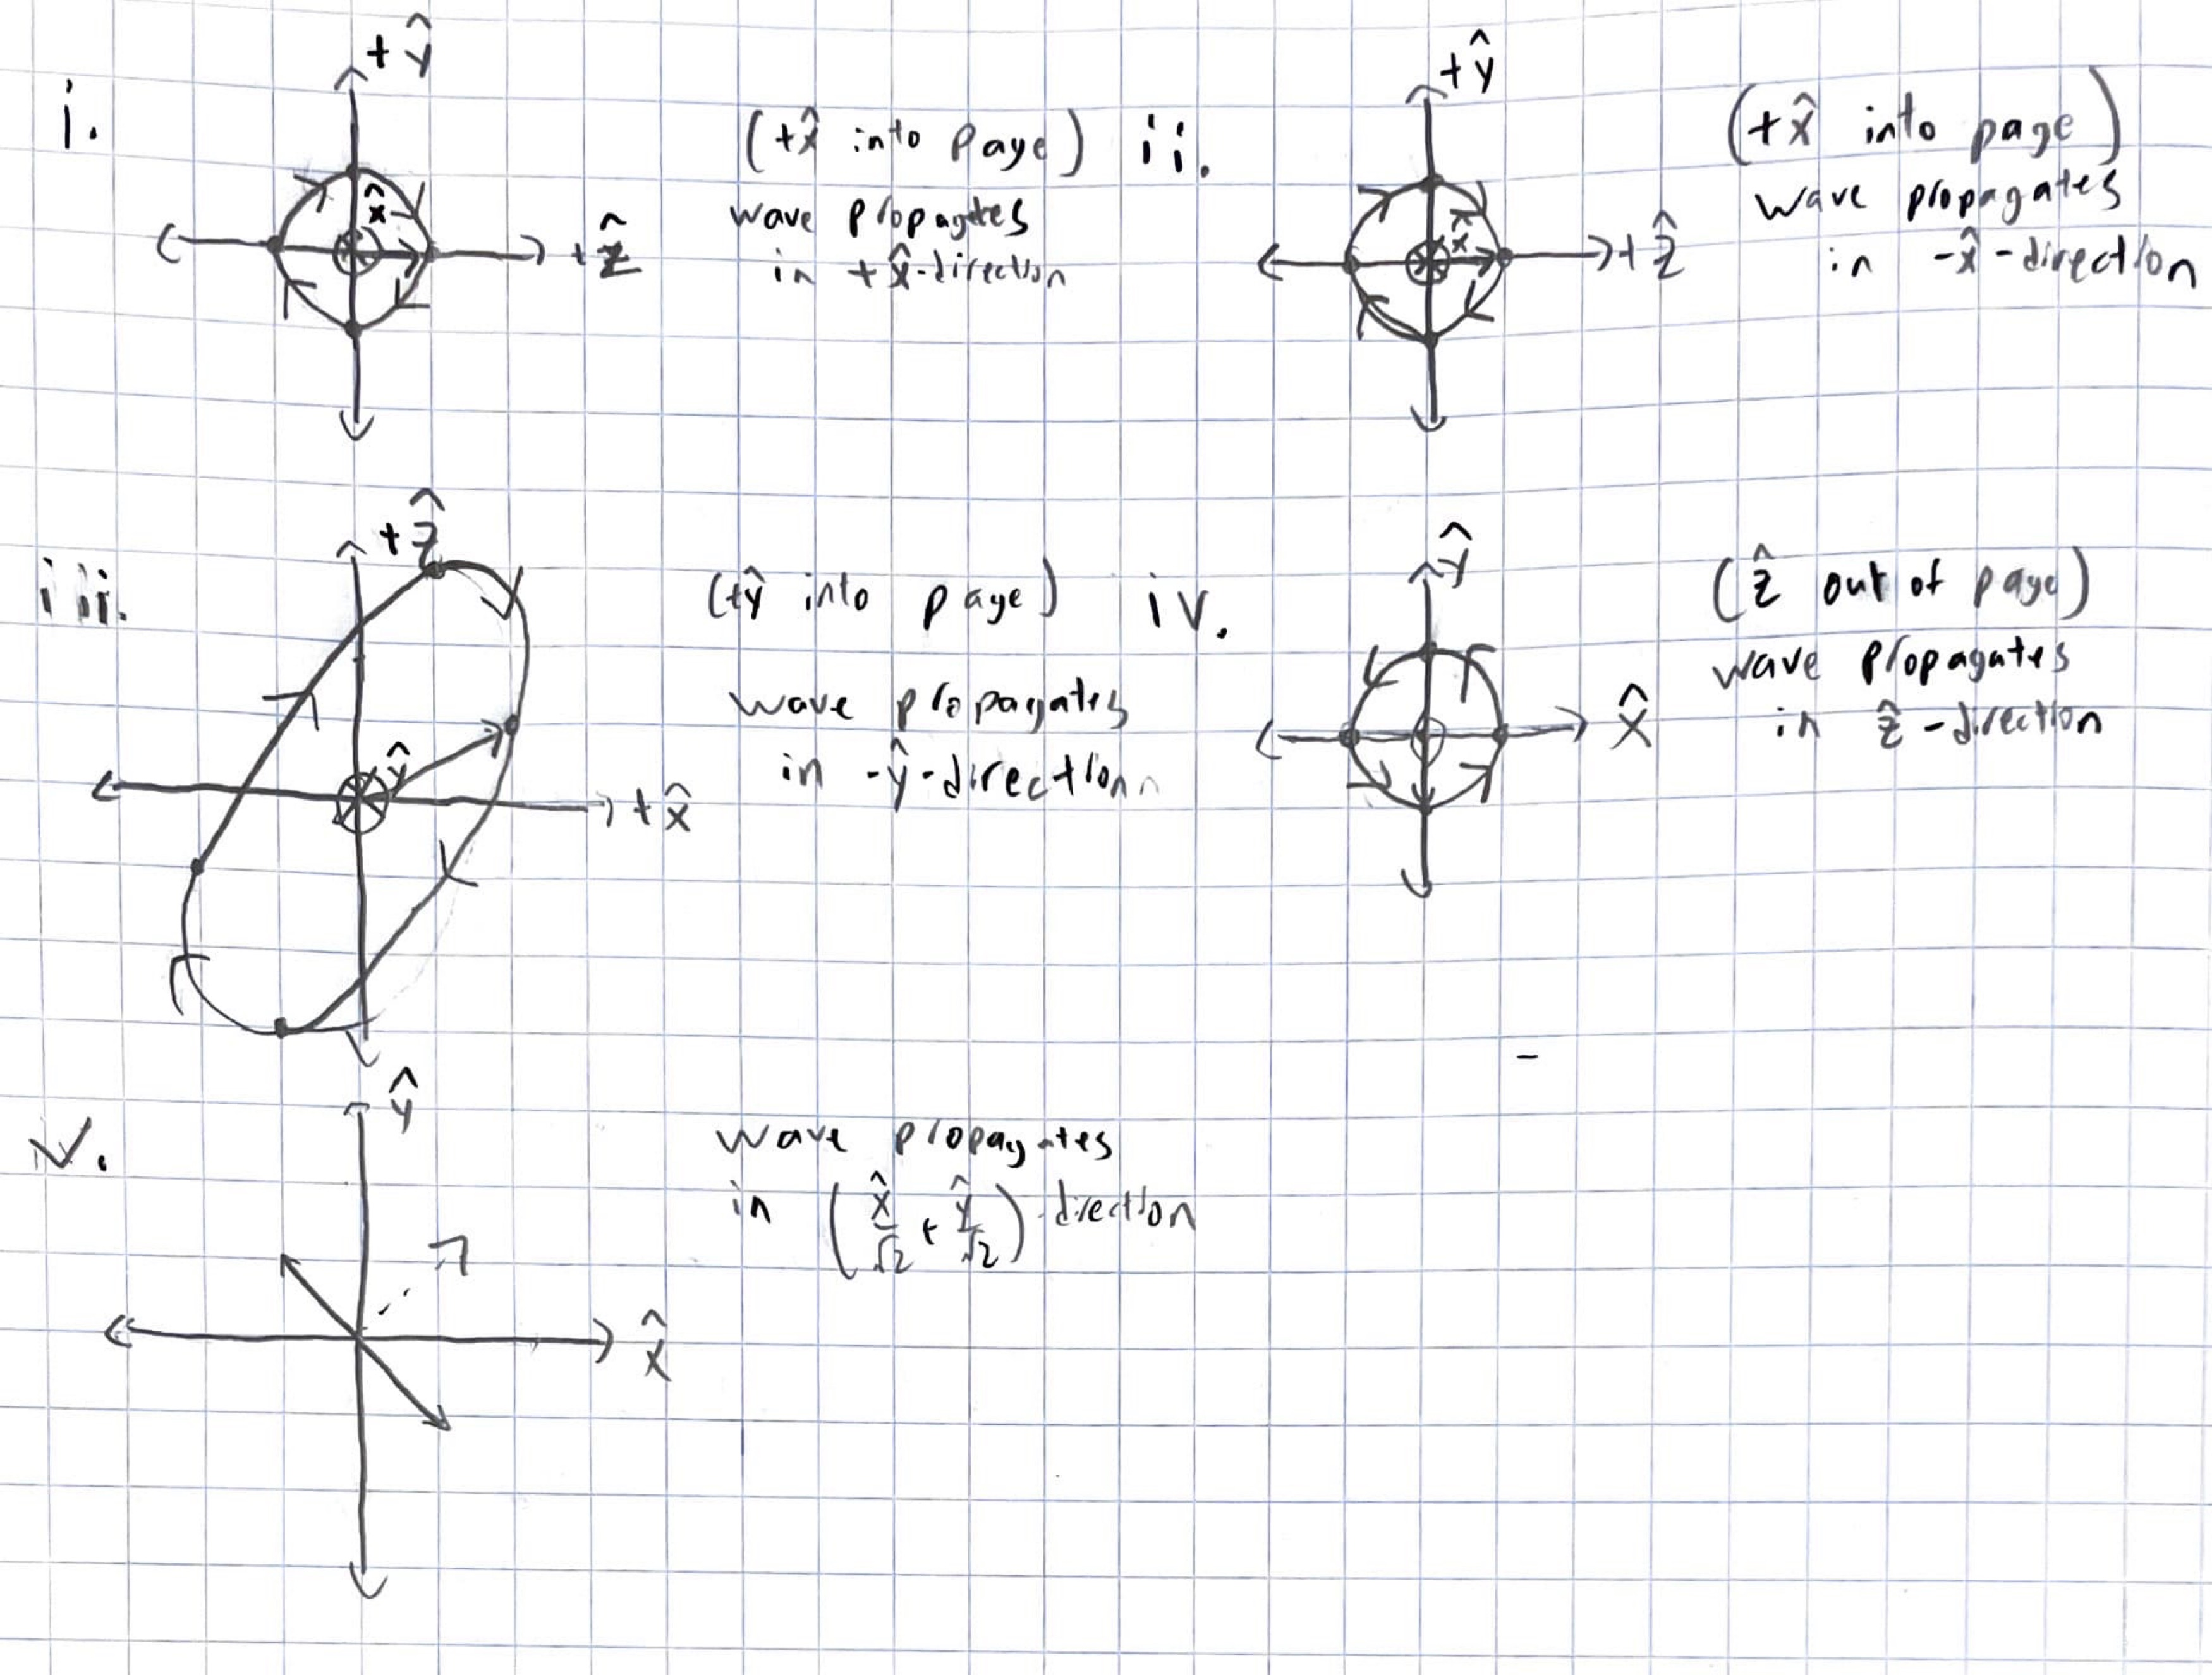
\includegraphics[width = 5in]{images/IMG_3957.jpg}

		\item [b.]
		Yes, it is a transverse wave because the electric field (and magnetic field as well) oscillate perpendicular to the direction of wave propagation.

		Showing this mathematically, we can find the normal vectors of each to be the following.
		The direction of wave propagation is given by,
		\[\hat n = \frac{\hat x}{\sqrt{2}} + \frac{\hat y}{\sqrt{2}}\]
		The direction of the electric field, $\hat e$, is given by,
		\[\hat e = -\hat x + \hat y\]
		Taking the dot product of the two,
		\[\hat n \cdot \hat e = -\frac{1}{\sqrt{2}}+\frac{1}{\sqrt{2}}=0\]
		Thus, the two vectors are orthogonal and our initial statement is proved.
		\[\boxed{\text{Yes.}}\]

		\item [c.]
		The time-averaged power flow per unit area is found by taking the time-average of the complex Poynting vector, $\langle \vec S(\vec r, t)\rangle$. 
		Through some trivial complex analysis, we find that this is equivalent to,
		\[\langle \vec S_1(\vec r,t)\rangle = \frac{1}{2}\mathrm{Re}\left[\vec E(\vec r)\times \vec H'(\vec r)\right]\]
		For time-harmonic fields, we derived in lecture that,
		\[\nabla \times \vec E(\vec r)=-j\omega \mu_0\vec H(\vec r)\to \vec H(\vec r)=(\hat k \times \vec n)\frac{E_0}{\eta_0}e^{-j\vec k \cdot \vec r}\]
		where $\vec E(\vec r)=E_0e^{-j\vec k \cdot \vec r}\vec n$, and $\eta_0=\sqrt{\mu_0/\epsilon_0}$.
		Finding $\vec H_1(\vec r)$,
		\[\vec H_1(\vec r)=(\hat x)\times (\hat z + j\hat y)\frac{E_0}{\eta_0}e^{-jkx}=(-\hat y+j\hat z)\frac{E_0}{\eta_0}e^{-jkx}\]
		Taking the complex conjugate,
		\[\vec H_1'(\vec r)=(-\hat y - j\hat z)\frac{E_0}{\eta_0}e^{jkx}\]
		Then,
		\[\langle \vec S_1(\vec r, t)\rangle = \frac{1}{2}\mathrm{Re}\left[\vec E_1(\vec r)\times \vec H_1'(\vec r)\right]\]
		\[\langle \vec S_1(\vec r, t)\rangle = \frac{1}{2}\mathrm{Re}\left[(\hat z + j\hat y)\times (-\hat y - j\hat z)\frac{E_0^2}{\eta_0}\right]\]
		\[\langle \vec S_1(\vec r, t)\rangle = \frac{1}{2}\mathrm{Re}\left[2\hat x \frac{E_0^2}{\eta_0}\right]=\frac{E_0^2}{\eta_0}\hat x\]
		\[\boxed{\langle \vec S_1(\vec r, t)\rangle = \frac{E_0^2}{\eta_0}\hat x}\]
		Similarly, finding $\vec H_2(\vec r)$,
		\[\vec H_2(\vec r)=(\hat x)\times (2\hat z + 2j\hat y)\frac{E_0}{\eta_0}e^{-jkx}=(-2\hat y + 2j\hat z)\frac{E_0}{\eta_0}e^{-jkx}\]
		Taking the complex conjugate,
		\[\vec H_2'(\vec r)=(-2\hat y - 2j\hat z)\frac{E_0}{\eta_0}e^{jkx}\]
		Then,
		\[\langle \vec S_2(\vec r, t)\rangle = \frac{1}{2}\mathrm{Re}\left[\vec E_2(\vec r)\times \vec H_2'(\vec r)\right]\]
		\[\langle \vec S_2(\vec r, t)\rangle = \frac{1}{2}\mathrm{Re}\left[(2\hat z + 2j\hat y)\times (-2\hat y - 2j\hat z)\frac{E_0^2}{\eta_0}\right]\]
		\[\langle \vec S_2(\vec r, t)\rangle = \frac{1}{2}\mathrm{Re}\left[8\hat x \frac{E_0^2}{\eta_0}\right]=\frac{4E_0^2}{\eta_0}\hat x\]
		\[\boxed{\langle \vec S_2(\vec r, t)\rangle = 4\frac{E_0^2}{\eta_0}\hat x}\]
		Taking the superposition of the electric fields to find the total electric field $\vec E_T$,
		\[\vec E_T(\vec r)=\vec E_1(\vec r)+\vec E_2(\vec r)=3(\hat x+j\hat y)E_0e^{-jkx}\]
		Finding $\vec H_T(\vec r)$,
		\[\vec H_T(\vec r)=(\hat x)\times (3\hat z + 3j\hat y)\frac{E_0}{\eta_0}e^{-jkx}=(-3\hat y + 3j\hat z)\frac{E_0}{\eta_0}e^{-jkx}\]
		Taking the complex conjugate,
		\[\vec H_T'(\vec r)=(-3\hat y - 3j\hat z)\frac{E_0}{\eta_0}e^{jkx}\]
		Then,
		\[\langle \vec S_T(\vec r, t)\rangle = \frac{1}{2}\mathrm{Re}\left[\vec E_T(\vec r)\times \vec H_T'(\vec r)\right]\]
		\[\langle \vec S_T(\vec r, t)\rangle = \frac{1}{2}\mathrm{Re}\left[(3\hat z + 3j\hat y)\times (-3\hat y - 3j\hat z)\frac{E_0^2}{\eta_0}\right]\]
		\[\langle \vec S_T(\vec r, t)\rangle = \frac{1}{2}\mathrm{Re}\left[18\hat x \frac{E_0^2}{\eta_0}\right]=\frac{9E_0^2}{\eta_0}\hat x\]
		\[\boxed{\langle \vec S_T(\vec r, t)\rangle = 9\frac{E_0^2}{\eta_0}\hat x}\]
		We notice that $\langle \vec S_T(\vec r, t)\rangle \neq \langle \vec S_1(\vec r, t)\rangle + \langle \vec S_2(\vec r, t)\rangle$.
		Thus, the power flow of the superposition is not equal to the sum of the individual waves' power flows.
		This is because when we find the power flow, it involves taking the real part of the complex Poynting vector.
		Thus, when we sum power flows, we are essentially taking the sum of the real parts of the two complex Poynting vectors.
		However, light interference is inherently a process that involves superpositions in $\mathbb{C}$.
		In other words, when we sum the power flows, we are ignoring the interference of the imaginary parts of the complex Poynting vector, which may affect its time-averaged quantity.
		By first taking the superposition of the two plane waves, we include the imaginary parts of the complex Poynting vector, which causes the delta between $\langle \vec S_T(\vec r, t)\rangle$ and $\langle \vec S_1(\vec r,t)\rangle+\langle \vec S_2(\vec r,t)\rangle$.


	\end{enumerate}

	\item [5.2]
	\begin{enumerate}
		\item [a.]
		We can express $\vec E(z,t)$ in phasor format as,
		\[\vec E(\vec r,t)=\mathrm{Re}\left[\vec E(\vec r)e^{j\omega t}\right]\]
		For a general plane wave, the phasor is given by, $\vec E(\vec r)=E_0e^{-j\vec k \cdot \vec r}\hat n$.
		Substituting this in,
		\[\vec E(\vec r, t)=\mathrm{Re}\left[E_0e^{-j\vec k \cdot \vec r}\hat n e^{j\omega t}\right]\]
		Going back to the original equation, we can express $\vec E(z,t)$ as,
		\[\vec E(z,t)=\mathrm{Re}\left[10e^{-j(2\pi z)}\hat x e^{j(4\pi \cdot 10^8t)}\right]\:\mathrm{V/m}\]
		Through direct comparison, we find that $\vec k \cdot \vec r = 2\pi z$, where $\vec r = z\hat z$.
		Thus, $\vec k = 2\pi \hat z$.
		We know that the units of $\vec k$ must 'cancel out' the units of $\vec r$ because an exponential cannot have units.
		Since $\vec r$ has units of meters, $\vec k$ must have units of $\mathrm{m}^{-1}$, yielding $\vec k = (2\pi \hat z)\: \mathrm{m}^{-1}$.
		We know that $\lambda = \frac{2\pi}{\|k\|}=1 \: \mathrm{m}$.
		Again, through direct comparison, we find that, $\omega = 4\pi \cdot 10^8$.
		We know that the units of $\omega$ must 'cancel out' the units of $t$ because an exponential cannot have units.
		Since $t$ has units of seconds, $\omega$ must have units of $\mathrm{s}^{-1}$, yielding $\omega = 4\pi\cdot 10^8 \: \mathrm{s^{-1}}$.
		We know that $\omega$ and $f$ are related by $\omega = 2\pi f \to f = \omega/2\pi$.
		Thus, $f=2 \cdot 10^8 \: \mathrm{Hz}$.
		We know that the wave velocity $\vec v$ is given by,
		\[\vec v= \frac{\omega}{\|k\|}\hat r = \lambda f \hat r = 2\cdot 10^8 \hat z \: \mathrm{m/s}\]
		Thus, we have,
		\[\boxed{\begin{cases}
			\vec k = (2\pi \hat z)\: \mathrm{m^{-1}} \\ 
			\lambda = 1\: \mathrm{m} \\ 
			\omega = 4\pi \cdot 10^8 \: \mathrm{s^{-1}} \\ 
			f = 2 \cdot 10^8 \: \mathrm{Hz} \\ 
			\vec v= (2\cdot 10^8 \hat z)\: \mathrm{m/s}
		\end{cases}}\]

		\item [b.]
		Faraday's Law tells us that,
		\[\nabla \times \vec E = -\frac{\partial \mu_0 \vec H}{\partial t}\]
		Using phasor expressions, we find that,
		\[\nabla \times \vec E(\vec r) = -j\omega \mu_0\vec H(\vec r)\]
		\[\to -j\vec k \times \vec E(\vec r)=-j\omega \mu_0\vec H(\vec r)\]
		\[\to \vec H(\vec r)=\frac{1}{\omega \mu_0}\vec k \times \vec E(\vec r)\]
		From the previous part, through direct comparison, we find that,
		\[\vec E(z) = 10e^{-j(2\pi z)}\hat x\]
		Thus, substituting known expressions in, (temporarily omit units here because everything is in SI units)
		\[\vec H(z)=\frac{1}{\omega \mu_0}((2\pi \hat z) \times \hat x)\cdot (10e^{-j(2\pi z)})\]
		\[\vec H(z)=\frac{1}{\omega \mu_0}(2\pi \hat y)\cdot (10e^{-j(2\pi z)})\]
		Substituting values for $\omega$ and $\mu_0$, we find that,
		\[\vec H(z)=\left[\frac{1}{8\pi}e^{-j(2\pi z)}\hat y\right] \: \mathrm{A/m}\]
		Fitting this in the form of,
		\[\vec H(\vec r)=(\hat k \times \hat n)\frac{1}{\eta}E_0e^{-j\vec k \cdot \vec r}\]
		\[\to \vec H(z)=\hat y\frac{1}{80\pi}10e^{j(2\pi z)}\]
		Thus, $\eta = 80\pi\:\Omega$.
		By definition, 
		\[\eta=\sqrt{\mu_0/\epsilon}\to \frac{\mu_0}{\epsilon}=\eta^2 \to \epsilon = \frac{\mu_0}{\eta^2}=1.989\cdot 10^{-11}\:\mathrm{F/m}\]
		We then have,
		\[\boxed{\begin{cases}
			\vec H(z)=\left[\frac{1}{8\pi}e^{-j(2\pi z)}\hat y\right] \: \mathrm{A/m} \\ 
			\eta = 80 \pi \: \Omega \\ 
			\epsilon = 1.989 \cdot 10^{-11} \: \mathrm{F/m}
		\end{cases}}\]


	\end{enumerate}

	\item [5.3]
	\begin{enumerate}
		\item [a.]
		Calculating the characteristic values $\omega \tau_d$ for both of the frequencies,
		\[\omega \tau_d = \omega \frac{\epsilon}{\sigma}\]
		Starting with $10 \: \mathrm{kHz}$,
		\[(2\pi \cdot 10 \: \mathrm{kHz})\cdot \frac{10\epsilon_0}{5\cdot 10^{-3}\:\mathrm{S/m}}=2\pi\cdot \frac{10^5 \epsilon_0}{5\cdot 10^{-3}}=2\pi \cdot \frac{8.85\cdot 10^{-4}}{5}=0.00111 \ll 1\]
		Thus, at $10\:\mathrm{kHz}$, the ground is a good conductor (imperfect metal).
		Similarly, using $100 \: \mathrm{MHz}$,
		\[(2\pi \cdot 100 \: \mathrm{MHz})\cdot \frac{10\epsilon_0}{5\cdot 10^{-3}\:\mathrm{S/m}}=11.121 \gg 1\]
		Thus, at $100 \: \mathrm{MHz}$, the ground is a bad conductor (lossy dielectric).
		\[\boxed{\begin{cases}
			10 \: \mathrm{kHz}\to & \text{good conductor} \\ 	
			100 \: \mathrm{MHz}\to & \text{bad conductor} \\ 	
		\end{cases}}\]

		\item [b.]
		For a conducting medium, we have the expression of,
		\[\nabla \times \vec H = \vec J + \frac{\partial \epsilon \vec E}{\partial t}=\sigma \vec E +\frac{\partial \epsilon \vec E}{\partial t}\]
		Using the time-harmonic field and phasor expressions, we find that,
		\[\nabla \times \vec H(\vec r) = \sigma \vec E + j\omega \epsilon \vec E(\vec r)\]
		We can then define $\epsilon_{\mathrm{eff}}$ such that,
		\[\nabla \times \vec H(\vec r) = j\omega \epsilon_{\mathrm{eff}}\vec E(\vec r)\]
		where,
		\[\epsilon_{\mathrm{eff}}=\epsilon\left(1-j\frac{\sigma}{\omega \epsilon}\right)\]
		Substituting this into the wave equation, we find that,
		\[\nabla^2 \vec E(\vec r)=-\omega^2\mu_0\epsilon_{\mathrm{eff}}\vec E(\vec r)\]
		Since $\nabla^2 \vec E(\vec r)=j\vec k \cdot j\vec k = -k^2$,
		\[k^2=\omega^2\mu_0\epsilon_{\mathrm{eff}}\]
		We know that the time averaged power per unit area, $\langle \vec S(\vec r, t)\rangle$ is given by,
		\[\langle \vec S(\vec r, t)\rangle = \frac{1}{2}\mathrm{Re}\left[\vec E(\vec r)\times \vec H'(\vec r)\right]\]
		Suppose we have $\vec E(\vec r)=E_0e^{-jkz}\hat x$.
		Then, finding the magnetic field,
		\[\nabla \times \vec E(\vec r) = -\frac{\partial \mu_0 \vec H(\vec r)}{\partial t}=-j\omega \mu_0 \vec H(\vec r)\]
		\[-jk\hat z \times \vec E(\vec r)=-j\omega \mu_0\vec H(\vec r)\]
		\[\to \vec H(\vec r)=\frac{k}{\omega \mu_0}E_0e^{-jkz}\hat y\]
		Separating $k$ into real and imaginary components via $k=k'-jk''$, for the fields,
		\[\vec E(\vec r)=E_0e^{-j(k'-jk'')z}\hat x=E_0e^{-jk'z}e^{-k''z}\hat x\]
		\[\vec H(\vec r)=\frac{k'-jk''}{\omega \mu_0}E_0e^{-jk'z}e^{-k''z}\hat y\]
		Taking the complex conjugate,
		\[\vec H'(\vec r)=\frac{k'+jk''}{\omega\mu_0}E_0e^{jk'z}e^{-k''z}\hat y\]
		Then,
		\[\vec E(\vec r)\times \vec H'(\vec r)=E_0^2\frac{k'+jk''}{\omega \mu_0}e^{-2k''z}\hat z\]
		Now finding the time-averaged power,
		\[\langle \vec S(\vec r,t )\rangle = \frac{1}{2}\mathrm{Re}\left[\vec E(\vec r)\times \vec H'(\vec r)\right]=\frac{E_0^2}{2}\left(\frac{k'}{\omega\mu_0}\right)e^{-2k''z}\hat z\]
		Thus, the time-averaged power reaches $1\%$ of its power when $e^{-2k''z_p}=0.01$.
		\[e^{-2k''z_p}=0.01 \to -2k''z_p=\ln(0.01)\to z_p=-\frac{\ln(0.01)}{2k''}\]
		We found that,
		\[k^2=\omega^2\mu_0\epsilon_{\mathrm{eff}} \to k=\omega \sqrt{\mu_0\epsilon_{\mathrm{eff}}}\]
		\[k=\omega\sqrt{\mu_0\epsilon\left(1-j\frac{\sigma}{\omega \epsilon}\right)}=\omega\sqrt{\mu_0\epsilon}\sqrt{1-j\frac{\sigma}{\omega \epsilon}}\]
		At $10\:\mathrm{kHz}$, the ground acts like a good conductor.
		We found that in this situation, $\sigma/\omega\epsilon \gg 1$, and then $k$ can be approximated as,
		\[k\approx\omega\sqrt{\mu_0\epsilon}\sqrt{-j\frac{\sigma}{\omega\epsilon}}=\omega \sqrt{\mu_0\epsilon}\sqrt{\frac{\sigma}{2\omega\epsilon}}(1-j)\]
		Then,
		\[k'' \approx \sqrt{\frac{\omega\mu_0\sigma}{2}}=0.01405\]
		Then,
		\[z_p = -\frac{\ln(0.01)}{2\cdot 0.01405}=163.889 \: \mathrm{m.}\]
		At $100 \: \mathrm{MHz}$, the ground acts like a bad conductor.
		We found that in this situation, $\sigma /\omega \epsilon \ll 1$, and then $k$ can be approximated as,
		\[k\approx\omega\sqrt{\mu_0\epsilon}\left(1-j\frac{\sigma}{2\omega \epsilon}\right)\]
		Then,
		\[k'' \approx \frac{\sigma}{2}\sqrt{\frac{\mu_0}{\epsilon}}=0.298\]
		Then,
		\[z_p = -\frac{\ln(0.01)}{2\cdot 0.298}=7.729 \: \mathrm{m.}\]
		Thus, we have the penetration depths $z_p$ of,
		\[\boxed{z_p = \begin{cases}
			163.889 \: \mathrm{m} & 10 \: \mathrm{kHz} \\ 
			7.729 \: \mathrm{m} & 100 \: \mathrm{MHz}	
		\end{cases}}\]

		\item [c.]
		The plot of the penetration depths versus frequency is given below.

		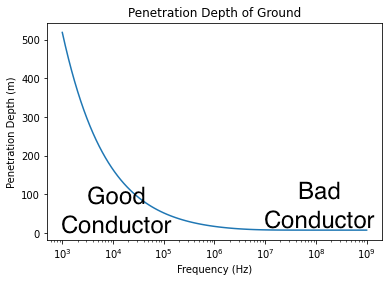
\includegraphics[width=5in]{images/plot1.png}


		\item [d.]
		Since the wave is reflected back up, it must travel $200\:\mathrm{m}$ in total through the isotropic medium.
		We assume that there is no losses due to reflection, and thus, we can model the percent of the power that comes back, $P$, as,
		\[P = e^{-400k''}\]
		If we want to image the smallest object possible, we want the highest frequency and smallest wavelength.
		By looking at the plot from part c above, we notice that the highest possibly frequency with a $200 \: \mathrm{m}$ penetration depth is at about $8 \: \mathrm{kHz}$ which is in the good conductor range.
		We found that in this range,
		\[k'' \approx \sqrt{\frac{\omega \mu_0\sigma}{2}}\]
		Substituting this into our expression for $P$,
		\[P=\mathrm{exp}\left(-400 \cdot \sqrt{\frac{\omega \mu_0\sigma}{2}}\right)=\mathrm{exp}\left(-400 \cdot \sqrt{\pi f \mu_0\sigma}\right)\]
		Trivially, by looking at this expression, we see that if we want to maximize $f$, we want to be at the minimal value of $P$ possible.
		The problem statement states that we must have $P\geq 0.01$.
		Thus, substituting this in,
		\[0.01\leq\mathrm{exp}\left(-400 \cdot \sqrt{\pi f \mu_0\sigma}\right)\]
		\[\to f\leq\left(-\frac{\ln(0.01)}{400}\right)^2\cdot \frac{1}{\pi\mu_0\sigma}\]
		\[\to f \leq 6.714 \: \mathrm{kHz}\]
		\[\boxed{f_{\mathrm{max}}=6.714 \: \mathrm{kHz}}\]





	\end{enumerate}
	
	
\end{enumerate}

		

\end{document}
